\documentclass[10pt,a4paper]{article}
\usepackage{amsmath}
\usepackage{amsfonts}
\usepackage{amssymb}
\usepackage{natbib}
\usepackage{graphicx}
\usepackage[left=2cm,right=2cm,top=2cm,bottom=2cm]{geometry}
\usepackage{arydshln}

\title{Revealing Transient Strain in Geodetic Data with the Radial Basis Function Finite Difference Method}
\author{Trever T. Hines and Eric A. Hetland}
\begin{document}

\maketitle


\section{Introduction}\label{sec:Introduction}
Crustal strain rates are fundementally important quantities for assessing seismic hazard. This is because the locations where strain is rapidly accumulating are the locations where we can expect strain energy to be released seismically.  It is then important to develop and improve upon methods for mapping strain in tectonically active regions because such maps could concievably feed into seismic hazard models such as UCERF3 \citep{Field2014}. 

Methods for estimating strain from geodetic data fall in one of two catagories.  There are model-based approaches which assume that strain is the result of loading on faults which have a known geometry, and there are data-based approaches which make no assumptions about the source of deformation.  We will exclusively consider data-based approaches in this paper.  The classic and simplest method for estimating strain is to assume that the strain rate is constant in time and spatially uniform within subnetworks of the geodetic data.  Linear least squares is then used to find the components of the strain rate tensor for each subnetwork \citep[e.g][]{Frank1966,Prescott1976,Savage1986,Feigl1990,Murray2000}. Several algorithms have been developed to improve upon this procedure. \citet{Shen1996} and \citet{Shen2015} discuss an algorithm where, instead of using the immediately adjacent stations to calculate strain at a position, the strain is computed with a weighted average over the entire network where the weighting is smaller for more distant stations.  Another strategy is to fit a set of interpolating basis functions to the deformation field and then compute the strain from the analytical derivative of the interpolant \citep[e.g.][]{Beavan2001,Tape2009,Sandwell2016}.  

The aforementioned studies have all been concerned with estimating long term strain rates. Time dependent strain would be useful for studying geophysical processes which occur over timescales of days to years such as slow slip events, postseismic relaxation, or volcanic deformation.  \citet{Ohtani2010} identified transient strain events by fitting a set of spatial wavelet basis functions to the deformation field at discrete time epochs, and a Kalman filtering strategy was used to ensure that the coefficients for each basis function varied smoothly in time. \citet{Holt2013} calculated time dependent strain by differentiating a bicubic interpolant that was fit to each epoch of a temporally smoothed deformation field. 

Each of the methods described above are designed to overcome two complications that arise in estimating deformation gradients: (1) geodetic data are noisy and differentiation will only amplify the noise and (2) geodetic data are not observed on a regular grid, which prevents the use of standard finite difference methods for computing derivatives. In this paper we demonstrate that both of these complications can be elegantly handled with the Radial Basis Function-Finite Difference (RBF-FD) method.  

The RBF-FD method was developed simultaneously and independently by \citet{Tolstykh2003}, \citet{Shu2003}, \citet{Cecil2004}, and \citet{Wright2006} as a computationally efficient way to solve large scale partial differential equations over irregular, multi-dimensional domains.  The RBF-FD method can be thought of as a generalization of the traditional finite difference method, where the node layout is no longer restricted to regular grids. Indeed, the RBF-FD method can be used to estimate derivates of discrete data located at arbitrary scattered positions in multi-dimensional space.  The RBF-FD method is particularly appealing because it is algorithmically simple, regardless of the domain shape or node layout, and also because the method has performed well in numerous benchmark tests \citep[and references therein]{Fornberg2015}.

In this paper, we do not use the RBF-FD method to solve a partial differential equation, but rather we use it to spatially smooth geodetic data and to compute deformation gradients. Our smoothing strategy can be viewed as a non-parametric, low-pass filter for scattered data where the degree of smoothness is controlled by a user specifies cutoff frequency. This can be contrasted with interpolation based methods where the resulting interpolant can be largely and perhaps unpredictably controlled by the choice of basis function. This process of smoothing and differentiating can be extended to estimate time dependent strain rates.  In that case, we first temporally smooth and differentiate GPS displacement time series to get time dependent velocities.  We then spatially smooth and differentiate the resulting velocities for each time epoch to get time dependent strain rates.  

The method proposed in this paper has numerous advantages which set it apart from other methods for computing strain rates. The method is computationally efficient and stable (there is no inversion of an ill-conditioned matrix).  There are no hyper parameters or penalty parameters that need to be tuned for each application.  As opposed to interpolation strategies such as \citet{Beavan2001}, \citet{Tape2009}, or \citet{Ohtani2010}, our method assumes that velocities are locally rather than globally continuous, which allows us to easily handle discontinuities resulting from, for example, a creeping fault. 

We begin this paper by summarizing the RBF-FD scheme and explaining how we construct differentiation matrices for scattered data. We then introduce the RBF-FD filter, which is used to smooth the observed geodetic data prior to differentiation.  We provide two real world demonstraitions of our method for calculating strain rates.  First we calculate the long term strain rates in Southern California from the CMM3 velocity data set \citep{Shen2011}, and we verify that our results are consistent with other studies. We then calculate time dependent strain rates in Cascadia from the GPS data provided by UNAVCO.  In Cascadia, we analyze strain resulting from slow slip events and compare it to the long term tectonic strain accumulation. Slow slip events are found to produce compression in the Olympic Peninsula, which is in addition to the compression resulting from tectonic loading.  Further south in Oregon, the slow slip events tend to release the compressional strain that is accumulated tectonically.  While similar conclusions have been drawn from fault slip inversions for slow slip events, it is important to recognize that slip inversion are the product of inverting an ill-conditioned matrix making it difficult to determine whether slip inferences are real or just an artifact of the inversion.  The strain rates presented in this paper are more direct observations and can be interpretted with a higher degree of confidence. 

\section{Method}\label{sec:Method}
\subsection{Differentiating Scattered Data}\label{sec:Differentiating}

In this section we briefly summarizing the RBF-FD method and we refer the reader to \citet{Wright2006} or \citet{Fornberg2015} for additional details. Consider a set of nodes $\mathbf{x} = \{x_i\}_{i=1}^N$ in $\mathbb{R}^d$ and a corresponding vector $\mathbf{u} = [u(x_1), ..., u(x_N)]^T$.  We want to find a differentiation matrix $\mathbf{L}$, such that $\mathbf{Lu}$ approximates the linear differential operator $\mathcal{L}$ acting on $u$ at $\mathbf{x}$.  For each node $x_i$ we approximate $\mathcal{L}[u(x)]\big|_{x=x_i}$ as a weighted sum of $\{u(x_j): j \in \mathcal{S}^i\}$ where $\mathcal{S}^i$ consist of $i$ and the indices for the $n-1$ nearest neighboring nodes to $x_i$.  The approximation can be written as

\begin{equation}\label{eq:RBFFDApprox}
\mathcal{L}[u(x)]\big|_{x=x_i} \approx \sum_{j \in \mathcal{S}^i} L_{ij} u(x_j)
\end{equation}
where $L_{ij}$ are the weights making up the differentiation matrix $\mathbf{L}$.  We refer to $x_i$ and its $n-1$ nearest neighbors as the stencil for $x_i$, and we denote the stencil as $\mathbf{x}^i = \{x_j : j \in \mathcal{S}^i\} = \{x^i_j\}_{j=1}^n$. The corresponding weights for each node in $\mathbf{x}^i$ are denoted as $\mathbf{w}^i = \{L_{ij} : j \in \mathcal{S}^i\} = \{w^i_j\}_{j=1}^n$.  We can then equivalently write eq. (\ref{eq:RBFFDApprox}) as 

\begin{equation}\label{eq:RBFFDApproxAlt}
\mathcal{L}[u(x)]\big|_{x=x_i} \approx \sum_{j=1}^n w^i_j u(x^i_j).
\end{equation}
Following \citet{Fornberg2015}, we find the components of $\mathbf{w}^i$, and thus also of $\mathbf{L}$, by solving the linear system of equations

\begin{equation}\label{eq:RBFFDWeights}
\left[
      \begin{array}{ccc:ccc}
      \phi(||x^i_1 - x^i_1||) & \cdots & \phi(||x^i_n - x^i_1||) & \psi_1(x^i_1) & \cdots & \psi_m(x^i_1) \\
      \vdots                  &        & \vdots                  & \vdots        &        & \vdots        \\   
      \phi(||x^i_1 - x^i_n||) & \cdots & \phi(||x^i_n - x^i_n||) & \psi_1(x^i_n) & \cdots & \psi_m(x^i_n) \\  
                              &        &                         &               &        &               \\ \hdashline 
                              &        &                         &               &        &               \\
      \psi_1(x^i_1)           & \cdots & \psi_1(x^i_n)           &  0            & \cdots & 0             \\
      \vdots                  &        & \vdots                  &  \vdots       &        & \vdots        \\   
      \psi_m(x^i_1)           & \cdots & \psi_m(x^i_n)           &  0            & \cdots & 0             \\       
      \end{array}
\right]
\left[
  \begin{array}{c}
  w^i_1  \\
  \vdots \\
  w^i_n  \\
         \\ \hdashline
         \\
  \lambda_1 \\
  \vdots    \\
  \lambda_m \\
  \end{array}
\right]  
=
\left[
  \begin{array}{c}
  \mathcal{L}\left[ \phi(||x - x^i_1||) \right] \big|_{x=x_i} \\
  \vdots                                                      \\
  \mathcal{L}\left[ \phi(||x - x^i_n||) \right] \big|_{x=x_i} \\
                                                              \\ \hdashline
                                                              \\  
  \mathcal{L}\left[ \psi_1(x) \right] \big|_{x=x_i}           \\
  \vdots                                                      \\
  \mathcal{L}\left[ \psi_m(x) \right] \big|_{x=x_i}           \\
  \end{array}
\right]
\end{equation}
for each stencil. In eq. (\ref{eq:RBFFDWeights}), $\phi$ is a radial basis function (RBF) which we describe below, $||\bullet||$ indicates the $L_2$ norm, $\{\psi_i\}_{i=1}^m$ are monomial basis functions that span the space of all $d$-dimensional polynomials with a specified degree $p$ (e.g. $\{1, x, y\}$ for $d=2$ and $p=1$), and $\{\lambda_i\}_{i=1}^m$ are parameters that are estimated along with $\mathbf{w}^i$ when eq. (\ref{eq:RBFFDWeights}) is inverted but they serve no purpose and can be discarded. 

Throughout this paper we use a cubic RBF for $\phi$,

\begin{equation}\label{eq:Cubic}
\phi(r) = r^3.
\end{equation}
The cubic RBF is an odd degree polyharmonic spline which has the benefit of being scale invariant and thus there is no scaling parameter that needs to be optimized, unlike for many other common choices of RBFs \citep[e.g.][]{Larsson2003}.  We note that the results presented in this paper remain virtually unchanged when we use other polyharmonic splines for $\phi$, which is consistent with the findings of \citet{Flyer2016}. 

We now elaborate on the stencil size, $n$, and the polynomial degree, $p$.  We choose $p$ to be equal to the degree of the derivative which we are approximating. This choice is based on the analysis of \citet{Flyer2016} and it ensures that eq. (\ref{eq:RBFFDApprox}) will converge to the true derivative as the distance between nodes decreases. The accuracy of eq. (\ref{eq:RBFFDApprox}) also generally improves with larger values of $n$, but at the expense of computational costs. We then choose $n$ to be large enough for eq. (\ref{eq:RBFFDApprox}) to converge. For the demonstrations in this paper, we find that $n=30$ is an appropriate choice.  It is worth noting that eq. (\ref{eq:RBFFDWeights}) cannot be inverted when the number of nodes is less than the number of monomial basis functions, $m$.  We then have a lower bound on $n$ which is $n \ge m = {{p+d}\choose{d}}$.   

\subsection{RBF-FD Filter}\label{sec:Filter}
We calculate strain rates by spatially differentiation geodetically observed velocities.  In order to differentiate noisy velocity data with the method described in Section \ref{sec:Differentiating}, we must first smooth the data. Existing strategies for smoothing scattered data can be classified as parametric and non-parametric approaches.  Parametric approaches involves fitting a set of basis functions to the data, perhaps using least-squares or regularized least-squares \citep[e.g.][]{Fasshauer2007}. Non-parametric approaches include kernel smoothing \citep[e.g.][]{Hastie1990} and Gaussian process regression \citep[e.g.][]{Rasmussen2006}. Kriging is among the better known examples of Gaussian process regression \citep{Matheron1963}.  Many of the wide variety of the existing strategies could surely produce a sufficiently smooth velocity field for us to calculate a coherent strain map. But since the intent of this paper is, in part, to demonstrate the utility of the RBF-FD method in geodesy, we present a smoothing strategy which we refer to as the RBF-FD filter.  This method is non-parametric and it offers several features which we find valuable.  The RBF-FD filter is computationally efficient and stable, it can be viewed as a low-pass filter with a well defined cutoff frequency, and we can easily specify discontinuities which we do not want to smooth across. In the following discussion of the RBF-FD filter, we seek to find a smoothed solution, $\mathbf{u}_\mathrm{post}$, from observed data, $\mathbf{u}_\mathrm{obs}$. We constrain $\mathbf{u}_\mathrm{post}$ with the observation equation

\begin{equation}\label{eq:Data}
  \mathbf{u}_\mathrm{post} = \mathbf{u}_\mathrm{obs} + \mathbf{\epsilon},\ \ \ \mathbf{\epsilon} \sim \mathcal{N}(\mathbf{0},\mathbf{C}_\mathrm{obs}),
\end{equation}
and the prior model

\begin{equation}\label{eq:Prior}
  \mathbf{u}_\mathrm{prior} \sim \mathcal{N}(\mathbf{0},\mathbf{C}_\mathrm{prior}),
\end{equation}
where $\mathbf{\epsilon}$ and $\mathbf{u}_\mathrm{prior}$ are considered to be Gaussian processes with zero mean and covariances $\mathbf{C}_\mathrm{obs}$ and $\mathbf{C}_\mathrm{prior}$ respectively.  The solution for $\mathbf{u}_\mathrm{post}$ minimizes the objective function  

\begin{equation}\label{eq:Objective}
||\mathbf{u}_\mathrm{post} - \mathbf{u}_\mathrm{obs}||_{\mathbf{C}_\mathrm{obs}}^2 + 
||\mathbf{u}_\mathrm{post}||_{\mathbf{C}_\mathrm{prior}}^2
\end{equation}
and is itself a Gaussian process with a distribution described by

\begin{equation}
  \mathbf{u}_\mathrm{post} \sim \mathcal{N}(\mathbf{\bar{u}}_\mathrm{post},\mathbf{C}_\mathrm{post}).
\end{equation}
We use $\mathbf{\bar{u}}_\mathrm{post}$ and $\mathbf{C}_\mathrm{post}$ to denote the mean and covariance of $\mathbf{u}_\mathrm{post}$ respectively.  Using Bayesian linear regression \citep{Tarantola2005} these values are found to be  

\begin{equation}\label{eq:GeneralSolution}
\begin{split}
  \mathbf{\bar{u}}_\mathrm{post} &= (\mathbf{C}_\mathrm{obs}^{-1} + 
                            \mathbf{C}_\mathrm{prior}^{-1})^{-1}
                            \mathbf{C}_\mathrm{obs}^{-1} \mathbf{u}_\mathrm{obs}
\\
\mathbf{C}_\mathrm{post} &= (\mathbf{C}_\mathrm{obs}^{-1} + 
                             \mathbf{C}_\mathrm{prior}^{-1})^{-1}.                          
\end{split}
\end{equation}
 
$\mathbf{C}_\mathrm{obs}$ is presumably well known, while $\mathbf{C}_\mathrm{prior}$ needs to be chosen based on an understanding of the underlying signal which we are trying to estimate. In Section \ref{sec:Smoothing1D} we discuss our choice for $\mathbf{C}_\mathrm{prior}$ and provide demonstrations with one-dimensional data.  The natural extension for $\mathbf{C}_\mathrm{prior}$ when dealing with $d$-dimensional data is discussed in Section \ref{sec:SmoothingND}.  

\subsubsection{Filtering in One Dimension}\label{sec:Smoothing1D}
For one-dimensional data we consider a prior which can be stated implicitly as

\begin{equation}\label{eq:ImplicitPrior1D}
  \mathbf{D}_{n} \mathbf{u}_\mathrm{prior} = \mathbf{q}, \ \ \ \mathbf{q} \sim \mathcal{N}(0,\lambda^2),
\end{equation}  
where $\mathbf{D}_n$ is an $n$'th order differentiation matrix, and $\mathbf{q}$ is a vector of white noise with constant variance $\lambda^2$. We leave the details of $\mathbf{D}_{n}$ unspecified for now. The inverse of the prior covariance matrix is

\begin{equation}\label{eq:ExplicitPrior1D}
\mathbf{C^{-1}_\mathrm{prior}}= \lambda^2\mathbf{D}_n^T\mathbf{D}_n,
\end{equation}
and the mean and covariance for the posterior are then 
\begin{equation}\label{eq:1DSolution}
\begin{split}
\mathbf{\bar{u}}_\mathrm{post} &= (\mathbf{C}_\mathrm{obs}^{-1} +   
                   \frac{1}{\lambda^2}\mathbf{D}_n^T\mathbf{D}_n)^{-1}\mathbf{C}_\mathrm{obs}^{-1}
                   \mathbf{u}_\mathrm{obs}
\\
\mathbf{C}_\mathrm{post} &= (\mathbf{C}_\mathrm{obs}^{-1} +   
                            \frac{1}{\lambda^2}\mathbf{D}_n^T\mathbf{D}_n)^{-1}.
\end{split}
\end{equation}
This solution is closely tied to several well established methods of smoothing.  For example, one can immediately recognize eq. (\ref{eq:1DSolution}) as an example of Tikhonov regularization \citep{Tikhonov1978}. We also note a similarity between eq. (\ref{eq:1DSolution}) and smoothing splines \citep{Wahba1990}.  To see this similarity, recall that a one-dimensional smoothing spline is defined as the function, $f(t)$, which minimizes,

\begin{equation}\label{eq:SmoothingSpline}
\sum_{i=1}^N \big((\mathbf{u_\mathrm{obs}})_i - f(t_i)\big)^2 + \alpha \int_{t_1}^{t_N} \left(f^{(n)}(t)\right)^2 dt,
\end{equation}
where $(\mathbf{u_\mathrm{obs}})_i$ is an observation at time $t_i$, $N$ is the number of observations, $\alpha$ is a smoothing parameter, and $f^{(n)}$ denotes the $n$'th time derivative of $f$.
In comparison, if we ignore data uncertainties (i.e. $\mathbf{C}_\mathrm{obs}=\mathbf{I}$), $\mathbf{\bar{u}}_\mathrm{post}$ is the discrete function which minimizes  

\begin{equation}\label{eq:1DObjective}
||\mathbf{u}_\mathrm{obs} - \mathbf{\bar{u}}_\mathrm{post}||_2^2 + \frac{1}{\lambda^2}||\mathbf{D}_n\mathbf{\bar{u}}_\mathrm{post}||_2^2.
\end{equation} 
If the sampling rate for $\mathbf{u}_\mathrm{obs}$ is constant and the penalty parameters are appropriately chosen then eq. (\ref{eq:1DObjective}) can be recognized as a discretized form of (\ref{eq:SmoothingSpline}).  We would thus expect $f(t)$ and $\mathbf{\bar{u}}_\mathrm{post}$ to be effectively identical.  The key difference between smoothing splines and the method presented here is that the former produces a globally smooth interpolant while we are only requiring local smoothness in our solution.  The benefits of imposing local smoothness are discussed in Section \ref{sec:Discontinuities}. 

We discuss the penalty parameter, $\lambda$. One common method for choosing an appropriate penalty parameter is generalized cross-validation \citep{Craven1979}, which yields a smoothed solution with the maximum predictive power. There is merit to using an entirely objective approach such as cross-validation, and this would be approriate if there is no prior knowledge of the signal's characteristic period. Otherwise, it may be better to chose a penalty parameter that damps out all the high frequency oscillations which are known to be noise. 

We demonstrate how $\lambda$ can be chosen so that frequencies greater than $\omega_c$ are attenuated.  We make the simplifying assumption that eq. (\ref{eq:1DSolution}) is a linear time-invariant (LTI) filter.  In doing so, we assume that $\mathbf{u}_\mathrm{obs}$ has a constant sampling rate, the data uncertainty is constant and uncorrelated ($\mathbf{C}_\mathrm{obs} = \sigma \mathbf{I}$), and $\mathbf{u}_\mathrm{prior}$ is periodic. We enforce periodicity in $\mathbf{u}_\mathrm{prior}$ by making $\mathbf{D}_n$ the periodic spectral differentiation matrix \citep[e.g.][]{Trefethen2000}. Under the discrete Fourier transform, $\mathbf{D}_n$ then has the properties 

\begin{equation}\label{eq:Property1}
  \mathcal{F}\left[\mathbf{D}_n \mathbf{g}\right]_k = (2\pi i\omega_k)^n \mathcal{F}\left[\mathbf{g}\right]_k
\end{equation}
and

\begin{equation}\label{eq:Property2}
  \mathcal{F}\left[\mathbf{D}^T_n \mathbf{g}\right]_k = (-2\pi i\omega_k)^n \mathcal{F}\left[\mathbf{g}\right]_k,
\end{equation}
where $\omega_k$ is the frequency domain variable and $\mathbf{g}$ is an arbitrary vector. With the LTI assumptions, the discrete Fourier transform of $\mathbf{\bar{u}}_\mathrm{post}$ is 

\begin{equation}\label{eq:1DFourierSoln1}
\mathcal{F}\left[\mathbf{\bar{u}}_\mathrm{post}\right]_k = \frac{\frac{1}{\sigma^2}}
                               {\frac{1}{\sigma^2} +                  
                                \frac{(2\pi\omega_k)^{2n}}{\lambda^2}}
                                \mathcal{F}\left[\mathbf{u}_\mathrm{obs}\right]_k.
\end{equation}
We make the change of variables 

\begin{equation}\label{eq:VariableChange}
\lambda^2 = (2\pi\omega_c)^{2n}\sigma^2
\end{equation}
which simplifies eq. (\ref{eq:1DFourierSoln1}) to

\begin{equation}\label{eq:1DFourierSoln2}
\mathcal{F}\left[\mathbf{\bar{u}}_\mathrm{post}\right]_k = \frac{1}
                                {1 + \left(\frac{\omega_k}{\omega_c}\right)^{2n}}
                                \mathcal{F}\left[\mathbf{u}_\mathrm{obs}\right]_k.        
\end{equation}
Based on eq. (\ref{eq:1DFourierSoln2}), we can recognize the frequency response of eq. (\ref{eq:1DSolution}) to be qualitatively similar to the frequency response for an $n$'th order low-pass Butterworth filter with cut-off frequency $\omega_c$.  In particular, the frequency response for eq. (\ref{eq:1DSolution}) is flat in the passband and decays log-linearly in the stopband (Figure \ref{fig:FrequencyResponse}).  In the limit as $n\to \infty$, eq. (\ref{eq:1DSolution}) becomes an ideal low-pass filter which removes all frequencies above $\omega_c$ and leaves lower frequencies unaltered.  

\begin{figure}
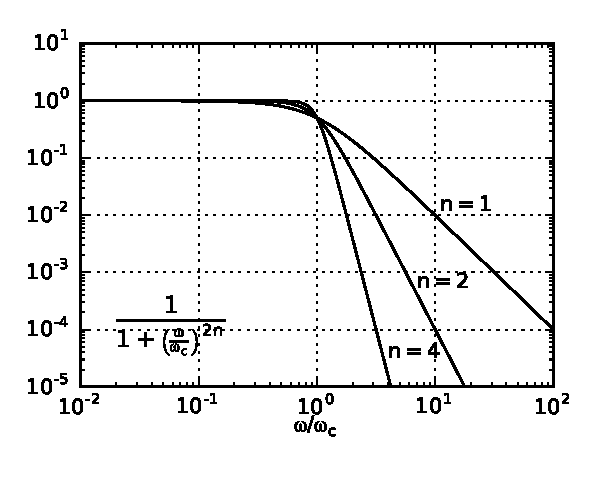
\includegraphics[scale=1.0]{figures/figure1}
\caption{Frequency response of the RBF-FD filter from eq. (\ref{eq:1DFourierSoln2}) for different values of $n$.}   
\label{fig:FrequencyResponse}
\end{figure}

The above Fourier analysis reveals how eq. (\ref{eq:1DSolution}) will behave under LTI assumptions.  For the GPS data considered in this paper, this assumption is not appropriate because neither the data uncertainties nor the sampling rates are constant. When the LTI conditions are not satisfied, it is no longer obvious how eq. (\ref{eq:1DSolution}) behaves or whether it can still be viewed as a low-pass filter with cutoff frequency $\omega_c$.  

\begin{figure}
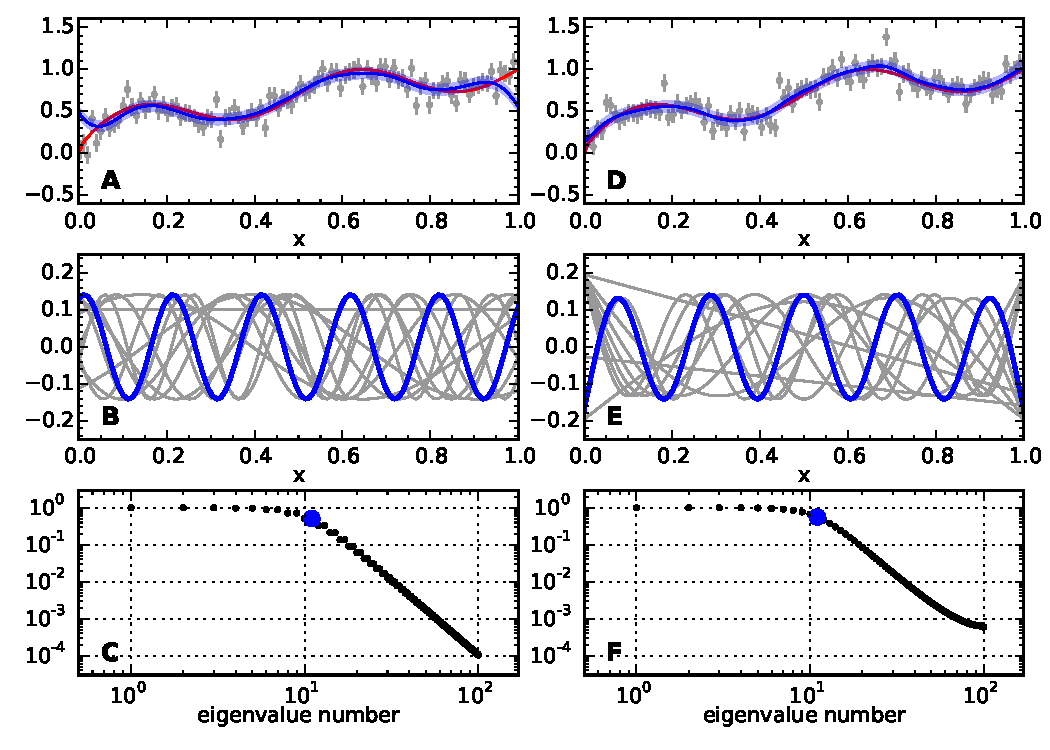
\includegraphics[scale=1.0]{figures/figure2}
\caption{eigenvectors and eigenvalues}   
\label{fig:Demo1}
\end{figure}

We explore the behavior of eq. (\ref{eq:1DSolution}) under more general conditions. We continue to substitute $\lambda$ in eq. (\ref{eq:1DSolution}) with eq. (\ref{eq:VariableChange}), which changes our free parameter to $\omega_c$. Since we are no longer assuming a constant variance, we replace $\sigma^2$ in eq. (\ref{eq:VariableChange}) with a characteristic variance, $\bar{\sigma}^2$, which we define as
         
\begin{equation}
\frac{1}{\bar{\sigma^2}} = \frac{1}{N} \mathrm{tr}\left(\mathbf{C}_\mathrm{obs}^{-1}\right),
\end{equation}
where $N$ is the number of observations.  We now write our smoothed solution as

\begin{equation}\label{eq:1DSolution2}
\begin{split}
\mathbf{\bar{u}}_\mathrm{post} &= (\mathbf{C}_\mathrm{obs}^{-1} +   
                   \frac{1}{(2\pi\omega_c)^{2n}\bar{\sigma}^2}\mathbf{D}_n^T\mathbf{D}_n)^{-1}
                   \mathbf{C}_\mathrm{obs}^{-1}
                   \mathbf{u}_\mathrm{obs}
\\
\mathbf{C}_\mathrm{post} &= (\mathbf{C}_\mathrm{obs}^{-1} +   
                            \frac{1}{(2\pi\omega_c)^{2n}\bar{\sigma}^2}\mathbf{D}_n^T\mathbf{D}_n)^{-1}.
\end{split}
\end{equation}
The behavior of eq. (\ref{eq:1DSolution2}) can be revealed by analyzing the eigen decomposition of the matrix mapping $\mathbf{u}_\mathrm{obs}$ to $\mathbf{\bar{u}}_\mathrm{post}$,

\begin{equation}\label{eq:Kernel}
\mathbf{K} = (\mathbf{C}_\mathrm{obs}^{-1} + 
              \frac{1}{(2\pi\omega_c)^{2n}\bar{\sigma}^2}\mathbf{D}_n^T\mathbf{D}_n)^{-1}\mathbf{C}_\mathrm{obs}^{-1}.
\end{equation}
The eigenvalues of $\mathbf{K}$, $\{s_1, \dots, s_N\}$, are real and bounded between 0 and 1.  The eigenvectors, $\{\mathbf{v}_1, \dots,\mathbf{v}_N\}$, are real and, when $\mathbf{K}$ is symmetric (e.g. when $\mathbf{C}_\mathrm{obs} = \sigma^2 \mathbf{I}$), form an orthogonal basis set.  Each eigenvalue, $s_i$,  describes the amount that $\mathbf{v}_i$ will be shrunk under the mapping $\mathbf{K}$.  The eigenvectors associated with eigenvalues close to 1 can then be interpretted as components which are retained in $\mathbf{\bar{u}}_\mathrm{post}$. When the LTI conditions are satisfied, the above Fourier analysis reveals that $\{\mathbf{v}_1, \dots, \mathbf{v}_N\}$ are a set of orthogonal sinusoids and $\{s_1, \dots s_N\}$ are the coresponding frequency responses from eq. (\ref{eq:1DFourierSoln2}) (Figure \ref{fig:Demo1}A-C). We show the eigen decomposition of $\mathbf{K}$ under non-LTI condtions where (1) $\mathbf{u}_\mathrm{prior}$ is aperiodic (Figure \ref{fig:Demo1}D-F), (2) $\mathbf{u}_\mathrm{prior}$ is aperiodic and the data uncertainties are not constant (Figure \ref{fig:Demo2}A-C), and (3) $\mathbf{u}_\mathrm{prior}$ is aperiodic and the data sampling rate is not constant (Figure \ref{fig:Demo2}D-F).  For case (1) and (3), the eigenvectors resemble sinusoids, except at the boundaries, and the eigenvalues decay in a manner that is consistent with the frequency response function in eq. (\ref{eq:1DFourierSoln2}). Namely, eq. (\ref{eq:1DFourierSoln2}) tells us that the eigenvectors associated with eigenvalues ${\geq}1/2$ are sinusoids with frequency ${\leq}\omega_c$.  For case (2), we  provide a demonstration where the data uncertainties are anomalously high from the time interval 0.2-0.5.  When looking outside of this time interval, the eigenvalues and eigenvectors are again consistent with the frequency response from eq (\ref{eq:1DFourierSoln2}). Within the time interval 0.2-0.5, the eigenvectors are elongated, which is desireable behavior because $\mathbf{u}_\mathrm{post}$ will not contort to fit the less certain observations. Since the frequency content of $\mathbf{u}_\mathrm{post}$ varies locally depending on the data uncertainty, we can only loosely view $\omega_c$ as a cutoff frequency. Nonetheless, we find in application that $1/\omega_c$ is a good predictor of the minimum feature wavelength retained in $\mathbf{u}_\mathrm{post}$, regardless of the data uncertainty or spacing.

\begin{figure}
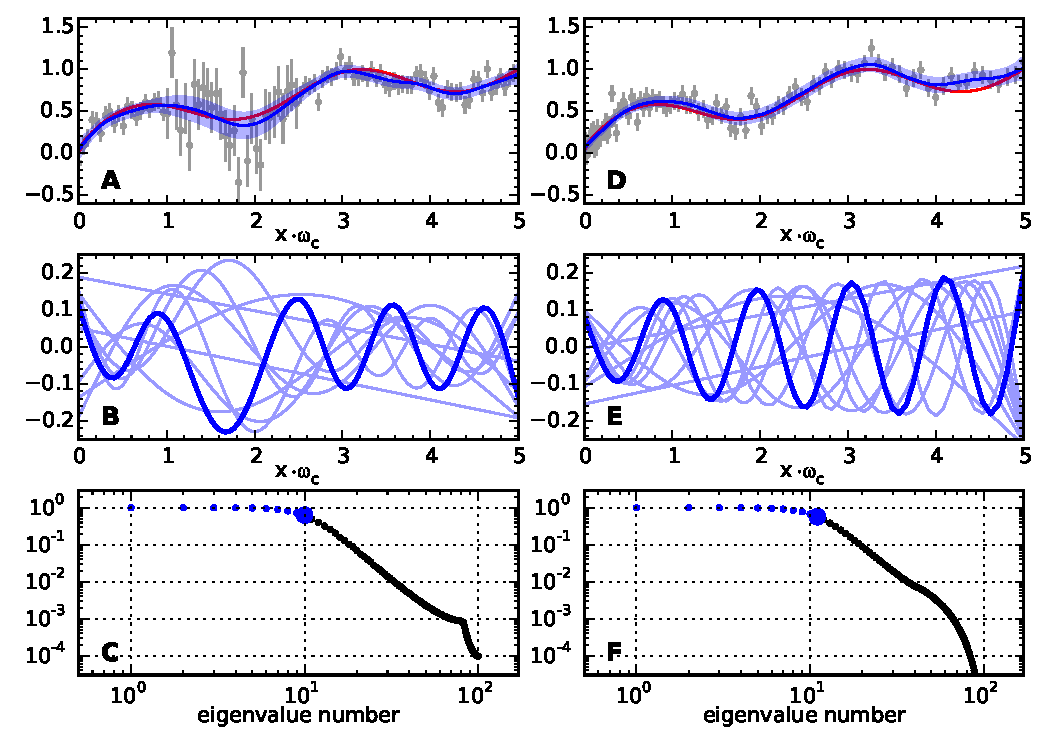
\includegraphics[scale=1.0]{figures/figure3}
\caption{eigenvectors and eigenvalues}   
\label{fig:Demo2}
\end{figure}

\subsubsection{Filtering in Higher Dimensions}\label{sec:SmoothingND} 
We expand our discussion to smoothing data which is observed in $d$-dimensional space. We now consider the prior model

\begin{equation}
  \mathbf{L}_n \mathbf{u}_\mathrm{prior} = \mathbf{q}, \ \ \ \mathbf{q} \sim \mathcal{N}(0,(2\pi\omega_c)^{2n}\bar{\sigma}^2)
\end{equation}  
where $\mathbf{L}_n$ is a differentiation matrix which approximates the operation 

\begin{equation}\label{eq:NDOperator}
  \sum_{i=1}^d\frac{\partial^n}{\partial x_i^n} 
\end{equation} 
and $n$ is an even integer. The variance chosen for $\mathbf{q}$ was motivated by the analysis in Section \ref{sec:Smoothing1D}. The mean and covariance of $\mathbf{u}_\mathrm{post}$ is now described by

\begin{equation}\label{eq:NDSolution}
\begin{split}
\mathbf{\bar{u}}_\mathrm{post} &= (\mathbf{C}_\mathrm{obs}^{-1} +   
                   \frac{1}{(2\pi\omega_c)^{2n}\bar{\sigma}^2}\mathbf{L}_n^T\mathbf{L}_n)^{-1}\mathbf{C}_\mathrm{obs}^{-1}
                   \mathbf{u}_\mathrm{obs}
\\
\mathbf{C}_\mathrm{post} &= (\mathbf{C}_\mathrm{obs}^{-1} +   
                            \frac{1}{(2\pi\omega_c)^{2n}\bar{\sigma}^2}\mathbf{L}_n^T\mathbf{L}_n)^{-1}.
\end{split}
\end{equation}
If we again assume that the observation are regularly spaced, have constant variance, and $\mathbf{L}_n$ is the corresponding spectral differentiation matrix, then the $d$-dimensional discrete Fourier transform of $\mathbf{\bar{u}}_\mathrm{post}$ is 

\begin{equation}\label{eq:NDFourierSoln}
  \mathcal{F}\left[\mathbf{\bar{u}}_\mathrm{post}\right]_k = 
  \frac{1}{1 + \left(\sum_{i=1}^d \left(\frac{\omega_{i,k}}{\omega_c}\right)^n\right)^2} \mathcal{F}\left[\mathbf{u}_\mathrm{obs}\right]_k.
\end{equation}
The frequency response for eq. (\ref{eq:NDSolution}) can once again be recognized as a low-pass filter with cutoff frequency $\omega_c$.  In the limit as $n \to \infty$, the frequency response becomes a $d$-dimensional box which is zero for all the frequency tuples $(\omega_{1,k},\dots \omega_{d,k})$ which have at least one component whos magnitude is greater than $\omega_c$. 

In general, $\mathbf{L}_n$ can be constructed with the RBF-FD scheme described in Section \ref{sec:Differentiating}, which allows us to use eq. (\ref{eq:NDSolution}) to smooth irregularly spaced data.  When that data are irregularly spaced, or if any of the above mentioned idealized conditions are not satisfied, eq. (\ref{eq:NDSolution}) exhibits the same behavior noted in Section \ref{sec:Smoothing1D}. In particular, it can be verified through eigen decomposition that the frequency content of $\mathbf{\bar{u}}_\mathrm{post}$ is consistent with $\omega_c$, regardless of the spacing or uncertainty of $\mathbf{u}_\mathrm{obs}$.

   
\subsection{Accounting for Known Discontinuities}\label{sec:Discontinuities}
The RBF-FD filter from Section \ref{sec:Filter} and the RBF-FD differentiation scheme from Section \ref{sec:Differentiating} can both account for known discontinuities from, for example, a creeping fault segment.  When using the RBF-FD scheme to estimate the strain rate from a velocity field, it is important not to use stencils that includes stations which are on opposite sides of a creeping fault segment. Doing so could result in estimated strain rates which are erroneously high. The stencils should thus be constructed so that no two stations within a stencil form an edge which intersects the trace of the creeping segment.  We also construct stencils in this manner when forming the differentiation matrix $\mathbf{L}_n$ from eq. (\ref{eq:NDSolution}).  By doing so, the RBF-FD filter will not produce a solution that is incorrectly tapered across a known discontinuity.

We elaborate on the statistical implications for how we handle discontinuities for the RBF-FD filter.  When $\mathbf{L}_n$ is constructed with the RBF-FD scheme, we can interpret $\mathbf{u}_\mathrm{prior}$ as a Gaussian Markov random field \citep[e.g.][]{Rue2005}.  That is to say, if $\mathbf{u}_\mathrm{prior}$ is known at stations within a neighborhood of $x_i$ then $\mathbf{u}_\mathrm{prior}$ at station $x_i$ is conditionally independent of $\mathbf{u}_\mathrm{prior}$ outside of that neighborhood.  The neighborhood consists of all stations which share a stencil with $x_i$. Our strategy for handling discontinuities thus imposes conditional independence between $\mathbf{u}_\mathrm{prior}$ at any two stations which form an edge that intersects the trace of a creeping fault segment. 

\begin{figure}
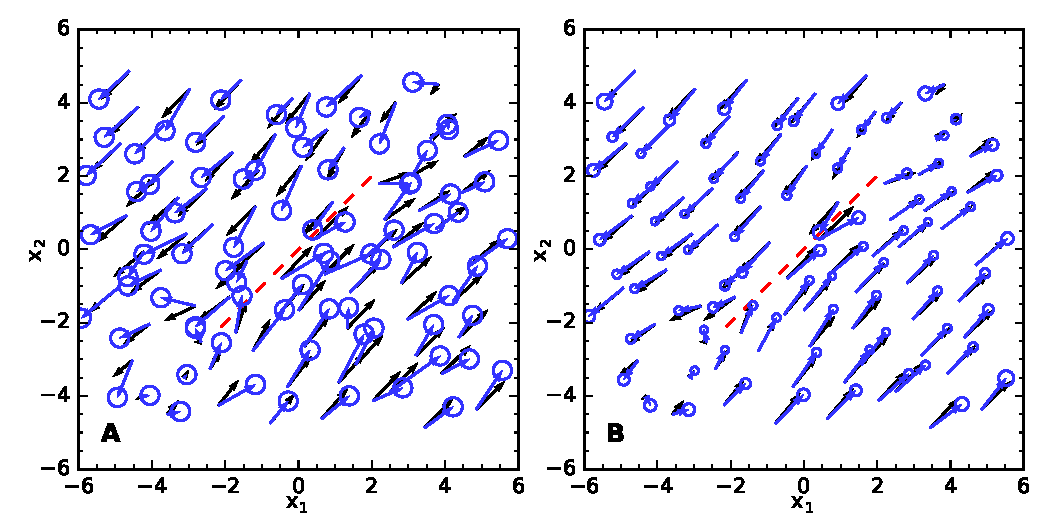
\includegraphics[scale=1.0]{figures/figure4}
\caption{eigenvectors and eigenvalues}   
\label{fig:Demo3}
\end{figure}

We demonstrate smoothing synthetic, scattered, two-dimensional vector data where there is a known discontinuity which we do not want to smooth across (Figure \ref{fig:Demo3}). The synthetic data is intended to simulates GPS velocities near a creeping fault segment. We generate the synthetic data with the elastic dislocation solution provided by \citet{Okada1992} and obscure the underlying signal with white noise. We smooth both directional components of the synthetic data independently with eq. (\ref{eq:NDSolution}). Figure \ref{fig:Demo3}A and \ref{fig:Demo3}B show the observed, $\mathbf{u}_\mathrm{obs}$, and smoothed, $\mathbf{u}_\mathrm{post}$, data compared to the true signal.  As noted in Section \ref{sec:Smoothing1D}, $\mathbf{u}_\mathrm{post}$ tends to have the highest uncertainty at the domain edges, and that is where $\mathbf{u}_\mathrm{post}$ does the poorest job at recovering the original signal.  Nonetheless, almost every smoothed datum in $\mathbf{u}_\mathrm{post}$ is an improvement over $\mathbf{u}_\mathrm{obs}$ at representing the underlying signal. 

\subsection{Numerical Notes}
Do not compute the inverse for upost!

This is well conditioned and lends itself well to iterative matrix solvers

The posterior covariance matrix is generally dense.  If memory does not permit the covariance matrix to be computed and one is only interested in the the data uncertainties then one can find the uncertainties by...

The posterior uncertainty does not account for error in L  

\section{Applications}\label{sec:Applications}

\subsection{Strain Rate in Southern California}\label{sec:ApplicationsSoCal}

We provide a demonstration in which we estimate the long term strain rates in southern California from the SCEC crustal motion map (CMM4)\citep{Shen2011}.  The crustal motion map provides an estimate of time-averaged horizontal velocities at over one thousand irregularly spaced points in sothern California.  The CMM4 is constrained by three decades of geodetic data and velocities have been corrected for coseismic and postseismic motions.  We independently smooth easting and northing components of the CMM4 velocities with the RBF-FD filter using a cutoff frequency $\omega_c=0.01\ \mathrm{km}^{-1}$. We do not smooth the velocities across the creeping segment of the San Andreas Fault (SAF), which extends from Parkfield to Hollister.  We show a comparison between the CMM4 velocities and smoothed velocities as supplementary material. We then differentiate the smoothed velocities with the RBF-FD scheme to find the velocity gradient and strain rates.  The estimated strain rates, complete with propagated uncertainties, are shown in Figure \ref{fig:SoCal1}, and it accurately illuminates well known features.  The strain map highlights the SAF and shows that the orientation of maximum shear strain runs parallel with the SAF strike \citep{Lisowski1991}.  Shear strain rates along the SAF are particularly high ($0.3-0.4$ micro-strain per year) in the Salton Trough and at the ends of the creeping segment. We can observe N-S contraction in the Los Angeles basin at a rate of $0.1-0.2$ micro-strain per year \citep{Shen1996,Argus1999,Argus2005}. We also observe a diffuse band of shear strain along the Eastern California shear zone (cite). These results are also consistent with the strain map by \citet{Shen2015}, which was derived from the same data set. 

\begin{figure}
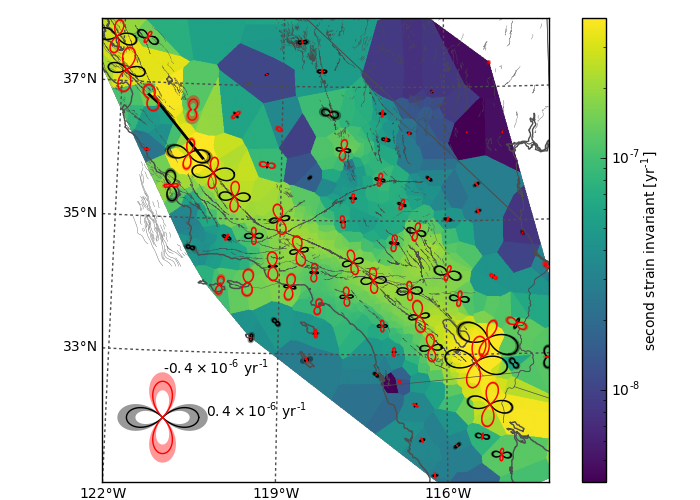
\includegraphics[scale=1.0]{figures/figure5.png}
\caption{Southern California strain map}   
\label{fig:SoCal1}
\end{figure}

The uncertainties on our strain estimates are shown as semi-transparent fields around the strain glyphs, and it may appear that our inferred strain rates are overly confident. In particular, the uncertainties on the estimated strain rates in Nevada are surprisingly low, given the sparse station coverage.  There are two sources of error which could potentially result in underestimated uncertainties: (1) we could have chosen a cutoff frequency that is too low for the geophysical signal that we are interested in and (2) the data coverage may be too sparse for the differentiation matrices to be accurate numerical approximations of the corresponding differential operators. The former is a well recognized bias inherent in any smoothing method \citep{Hastie1990}, and we address the latter here. Ideally, we would want the average distance between adjacent stations to be ${<}1/\omega_c$. Such a dense coverage would ensure that the differentiation matrix used to estimate the velocity gradient is sufficiently accurate. In this demonstration, the data spacing in Nevada is comparable to $1/\omega_c=100$ km. One remedy for the sparse coverage is to use the RBF-FD filter to interpolate the smoothed solution onto a finer grid of points and then find the velocity gradient of the denser smoothed data set. As suggested in Section \ref{sec:Filter}, the RBF-FD filter can be used for interpolation by treating the interpolation points as data with infinite uncertainty. Doing so will increase the accuracy of velocity gradient estimates, but at the expense of increased computational cost.  Figure \ref{fig:SoCal2}A shows a map of estimated strain rates where we improved the accuracy of velocity gradient estimate by interpolating the smoothed velocities on a grid with a ${\sim}5$ km spacing.  The inferred strain rates at points along the SAF, where the coverage is sufficiently dense, do not appear to be significantly improved by the added interpolation points. The uncertainties on the strain rates in Nevada are much higher, and likely more appropriate, when we included the interpolation points.

\begin{figure}
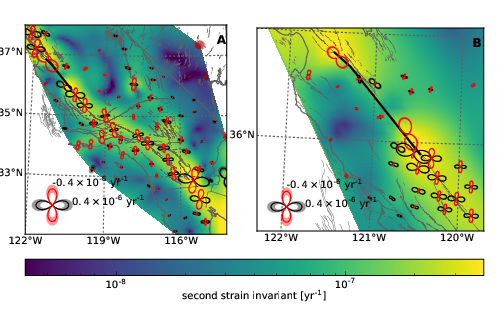
\includegraphics[scale=1.0]{figures/figure6.png}
\caption{Southern California strain map}   
\label{fig:SoCal2}
\end{figure}

In Figure \ref{fig:SoCal2}B, we highligh the creeping segment of the SAF, which is a notebly problematic area when trying to estimate strain rates in southern California \citep[e.g.][]{Sandwell2016}.  We find that the strain rate is greatest at the two ends of the creeping segment, near Parkfield and Hollister.  We are also able to resolve a quadrant pattern of extension and compression at the ends of the creeping segment. This strain pattern is consistent with what would be expected from an elastic dislocation model, giving us confidence that the inferred strain rates are accurate.

\subsection{Time Depenent Strain Rate in Cascadia}\label{sec:ApplicationsCascadia}

\citet{Dragert2001} first discovered slow slip events

Slow slip event depths from \citet{Dragert2001}, \citet{Wech2009}, \citet{Schmidt2010}, \citet{Bartlow2011} show slip concentrated at depths from 30 to 50 km detph.
 
Interseismic locking depths from \citet{Fluck1997}, \citet{Murray2000}, \citet{McCaffrey2007} and \citet{McCaffrey2013}, \citet{Burgette2009}, \citet{schmalzle2014} are consistent with a full locking down to about 20 km.

%Studies which simultaneously looked at intersesimic and ets are \citet{Holtkamp2010} and \citet{Schmalzle2014}
Studies which simultaneously modeled interseismic and ets are \citet{Holtkamp2010} and \citet{schmalzle2014}

\section{Discussion and Conclusion}\label{sec:Discussion}
% discuss potential applications for slip models

% discuss how we remove errors like reference frame and seasonals

% discuss how this can be used for tikhonov regularization

% we do not interpolate the strain field because it may introduce spurious artifacts Baxter2011

% Discuss similarities with PCA used in Dong2006 and common mode error by ...
% note that these errors are due to long wavelength features which get removed in strain calculations!!!
% see strain method by almendinger2007

% mention the scec geodetic transient exercise Lohman2013 and references therein

% Note that segalls 2016 paper mentions the gap between interseismic and sse

% mention howell2016, who said some crap about verticals, mention Hammond2016 so said more sensible crap about verticals

% note that this can be used for smoothing verticals, and compare it with burgette2009

\bibliographystyle{apalike}
\bibliography{mybib}  
 
\end{document}